%! Tex program = pdflatex
 
\documentclass[UTF8]{ctexart}
\CTEXsetup[format={\Large\bfseries}]{section}
\usepackage{amsmath}
\usepackage{ctex}
\usepackage{array}
\usepackage{ulem}
\usepackage{graphicx}
\usepackage{geometry}
\usepackage{multirow}
\usepackage{subfig}
\usepackage{float}
\usepackage{multicol}
\usepackage{multirow}
\usepackage{indentfirst}
\usepackage{makecell}
\geometry{papersize={21cm,29.7cm}}
\geometry{left=2.54cm,right=2.54cm,top=3.18cm,bottom=3.18cm}
\usepackage{fancyhdr}
\pagestyle{fancy}
\lhead{\today}
\chead{}
\rhead{2020011075}
\lfoot{清华大学}
\cfoot{\thepage}
\rfoot{物理实验B(2)}
\renewcommand{\headrulewidth}{0.4pt}
\renewcommand{\headwidth}{\textwidth}
\renewcommand{\footrulewidth}{0pt}
\usepackage{bm}
\begin{document}
\begin{titlepage}
    \begin{center}
		\quad \\
		\quad \\
        \quad \\
        \quad \\
        \quad \\
        \quad \\
		\kaishu \fontsize{30}{15} 光栅衍射
	\end{center}
	\vskip 10cm

    \begin{center}
        \begin{large}
        \begin{tabular}{cc}
        院\qquad 系:& ~~~~~~~~自动化系~~~~~~~~      \\
        \cline{2-2}\\
        班\qquad 级:& 自02班   \\
        \cline{2-2}\\
        学生姓名:& 彭程    \\
        \cline{2-2}\\
        学\qquad 号:&2020011075   \\
        \cline{2-2}\\
        组\qquad 号:& 双四下L    \\
        \cline{2-2}\\
        座~~位~~号:& \# 5    \\
        \cline{2-2}
        \end{tabular}
        \end{large}
        \end{center}

\end{titlepage}
\newpage
\tableofcontents
\newpage
\section{实验名称}
光栅衍射

\section{数据处理}

\subsection{不确定度推导}

由于:
$$
d=\frac{m \lambda}{\sin \varphi_{m}}  \nonumber\\
$$

故有:

$$
\ln d=\ln m+\ln \lambda-\ln \sin \varphi_{m} \nonumber\\
$$

而:


$$  
\frac{\partial \ln d}{\partial m}=\frac{1}{m} \nonumber\\
$$
$$  
\frac{\partial \ln d}{\partial \lambda}=\frac{1}{\lambda} \nonumber\\
$$
$$
\frac{\partial \ln d}{\partial \sin \varphi_{m}}=-\frac{1}{\sin \varphi_{m}} \nonumber
$$

所以有:

$$
\frac{\Delta d}{d}=\sqrt{\left(\frac{\Delta m}{m}\right)^{2}+\left(\frac{\Delta \lambda}{\lambda}\right)^{2}+\left(\frac{\Delta \sin \varphi_{m}}{\sin \varphi_{m}}\right)^{2}}=\sqrt{\left(\frac{\Delta m}{m}\right)^{2}+\left(\frac{\Delta \lambda}{\lambda}\right)^{2}+\left(\Delta \varphi_{m} \operatorname{ctg} \varphi_{m}\right)^{2}}
$$

即:
$$
\frac{\Delta d}{d}=\sqrt{\left(\frac{\Delta m}{m}\right)^{2}+\left(\frac{\Delta \lambda}{\lambda}\right)^{2}+\left(\Delta \varphi_{m} \operatorname{ctg} \varphi_{m}\right)^{2}}
$$

同理可得:
$$
\frac{\Delta \lambda}{\lambda}=\sqrt{\left(\frac{\Delta m}{m}\right)^{2}+\left(\frac{\Delta d}{d}\right)^{2}+\left(\Delta \varphi_{m} \operatorname{ctg} \varphi_{m}\right)^{2}}
$$

  由预习报告中关于不确定度的分析可以知道, $\varphi_{m}$  越大,  $\left(\frac{\Delta d}{d}\right)^{2}$  越小, 即  $\Delta d $ 越小, 故取衍射光级次尽量大。 又由于过高级次的光强较小的原因, 综合考虑,本次实验最终取衍射光谱级次$m=2$ 。


\subsection{光线垂直入射测光栅常数和光波波长}

\begin{figure}[H]
  \centering
  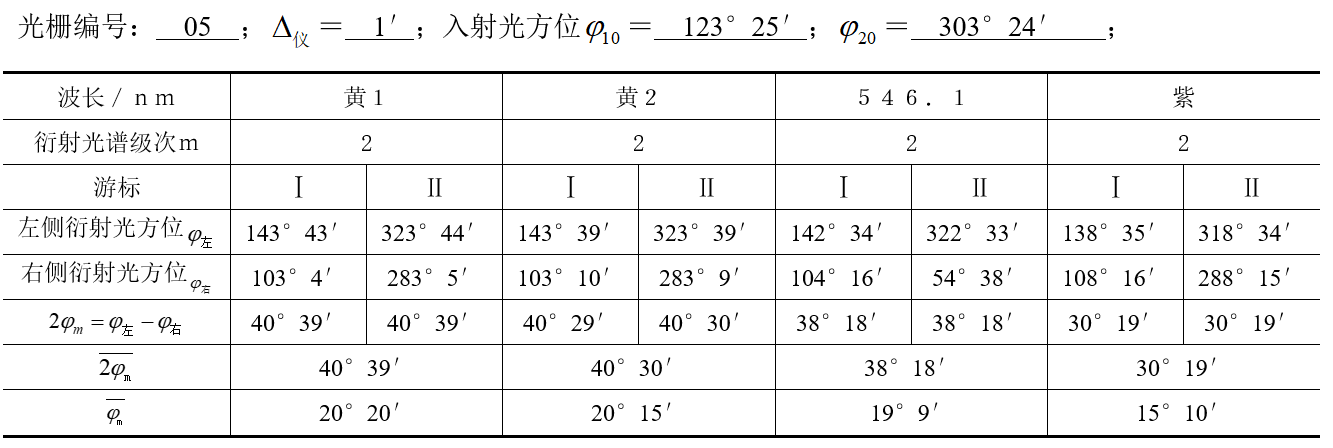
\includegraphics[scale=0.7]{表格1.png}
\end{figure}

由于:
$$
d \sin \varphi_{m}=m \lambda \\
$$

对于绿光: $ \lambda=546.1 \mathrm{~nm}, \varphi_{m}=19^{\circ}9' $

故代入公式得到:

$$
\mathrm{~d}=3329.4 \mathrm{~nm}
$$

由于 $\mathrm{~m}$  的不确定度为  0, 该条件下采用绿光的标准波长,故$\lambda $ 的不确定度非常小, 可忽略,代入之前推导出的不确定度公式有:

$$
\frac{\Delta d}{d}=\sqrt{\left(\frac{\Delta m}{m}\right)^{2}+\left(\frac{\Delta \lambda}{\lambda}\right)^{2}+\left(\frac{\Delta \sin \varphi_{m}}{\sin \varphi_{m}}\right)^{2}}=\sqrt{\left(\Delta \varphi_{m} \operatorname{ctg} \varphi_{m}\right)^{2}}
$$

而$\varphi_m$ 的不确定度来源为两次读数取平均值,故有:

$$
\Delta \varphi_m = \frac{1}{2}\sqrt{{2\Delta \mbox{仪} }^2} = 0.707'
$$

所以有:
$$
   \Delta d=d \Delta \varphi_{m} \operatorname{ctg} \varphi_{m}=3329.4 \times \frac{\pi \times 0.707}{60 \times 180} \times \operatorname{ctg} 19^{\circ}9'=2.0 \mathrm{~nm} 
$$

故:
$$
  \mathrm{d}=(3329.4 \pm 2.0) \mathrm{nm}
$$

  由计算出的  $\mathrm{d}=3329.4 \mathrm{~nm}$  和测得的各光线的  $\varphi_{m} $ 值计算出:

  紫光: $\varphi_{m}=15^{\circ} 10^{\prime} $
  $$
  \lambda=\frac{d \sin \varphi_{m}}{m}=435.5 \mathrm{~nm}
  $$

  黄1: $\varphi_{m}=20^{\circ} 20^{\prime} $
  $$
  \lambda=\frac{d \sin \varphi_{m}}{m}=578.5 \mathrm{~nm}
  $$

  黄2: $\varphi_{m}=20^{\circ} 15^{\prime} $
  $$
  \lambda=\frac{d \sin \varphi_{m}}{m}=576.2 \mathrm{~nm}
  $$

  计算  $\Delta \lambda$  的过程如下:
  之前推导出的不确定度公式有:
   $$
   \frac{\Delta \lambda}{\lambda}=\sqrt{\left(\frac{\Delta d}{d}\right)^{2}+\left(\frac{\Delta m}{m}\right)^{2}+\left(\Delta \varphi_{m} \operatorname{ctg} \varphi_{m}\right)^{2}} 
   $$

   而:
   $$
   \Delta \varphi_{m}=\frac{1}{2} \sqrt{2 \Delta_{\text {仪 }}^{2}}=0.707^{\prime} \quad \Delta m=0
   $$
 
   所以有:
  
   紫光: 
   \begin{align}
    \frac{\Delta \lambda}{\lambda}&=\sqrt{\left(\frac{\Delta d}{d}\right)^{2}+\left(\Delta \varphi_{m} \operatorname{ctg} \varphi_{m}\right)^{2}}  \nonumber \\
    & = \sqrt{\left(\frac{2.0}{3329.4}\right)^{2}+\left(\frac{\pi \times 0.707}{60 \times 180} \times \operatorname{ctg} 15^{\circ}10'\right)^{2}} \nonumber \\
    & = 7.2 \times 10^{-4} \nonumber
   \end{align}

   
   $$ 
   \Delta \lambda=\lambda \cdot \frac{\Delta \lambda}{\lambda} = 0.3 \mathrm{~nm} 
   $$
   $$
   \quad \lambda=(435.5 \pm 0.3) \mathrm{nm} 
   $$

   黄1: 
   \begin{align}
    \frac{\Delta \lambda}{\lambda}&=\sqrt{\left(\frac{\Delta d}{d}\right)^{2}+\left(\Delta \varphi_{m} \operatorname{ctg} \varphi_{m}\right)^{2}}  \nonumber \\
    & = \sqrt{\left(\frac{2.0}{3329.4}\right)^{2}+\left(\frac{\pi \times 0.707}{60 \times 180} \times \operatorname{ctg} 20^{\circ}20'\right)^{2}} \nonumber \\
    & = 6.9 \times 10^{-4} \nonumber
   \end{align}

   
   $$ 
   \Delta \lambda=\lambda \cdot \frac{\Delta \lambda}{\lambda} = 0.4 \mathrm{~nm} 
   $$
   $$
   \quad \lambda=(578.5 \pm 0.4) \mathrm{nm} 
   $$

   黄2: 
   \begin{align}
    \frac{\Delta \lambda}{\lambda}&=\sqrt{\left(\frac{\Delta d}{d}\right)^{2}+\left(\Delta \varphi_{m} \operatorname{ctg} \varphi_{m}\right)^{2}}  \nonumber \\
    & = \sqrt{\left(\frac{2.0}{3329.4}\right)^{2}+\left(\frac{\pi \times 0.707}{60 \times 180} \times \operatorname{ctg} 20^{\circ}15'\right)^{2}} \nonumber \\
    & = 6.9 \times 10^{-4} \nonumber
   \end{align}

   $$ 
   \Delta \lambda=\lambda \cdot \frac{\Delta \lambda}{\lambda} = 0.4 \mathrm{~nm} 
   $$

   $$
   \quad \lambda=(576.2 \pm 0.4) \mathrm{nm} 
   $$

\noindent 综上所述:

根据绿光波长计算出的光栅常数为:
$$
  \mathrm{d}=(3329.4 \pm 2.0) \mathrm{nm}
$$
  
根据光栅常数计算其他光的波长为:

紫光:
$$
\quad \lambda=(435.5 \pm 0.3) \mathrm{nm} 
$$

偏差为:
$$
\delta = \frac{\lambda_{\mbox{紫}}-\lambda}{\lambda_{\mbox{紫}}}=0.07\%
$$

黄1:
$$
\quad \lambda=(578.5 \pm 0.4) \mathrm{nm} 
$$

偏差为:
$$
\delta = \frac{\lambda_{\mbox{黄1}}-\lambda}{\lambda_{\mbox{黄1}}}=0.10\%
$$


黄2:
   $$
   \quad \lambda=(576.2 \pm 0.4) \mathrm{nm} 
   $$

   偏差为:
   $$
   \delta = \frac{\lambda_{\mbox{黄2}}-\lambda}{\lambda_{\mbox{黄2}}}=0.14\%
   $$

\subsection{测量汞灯光谱中波长较短的黄线的波长}

\begin{figure}[H]
  \centering
  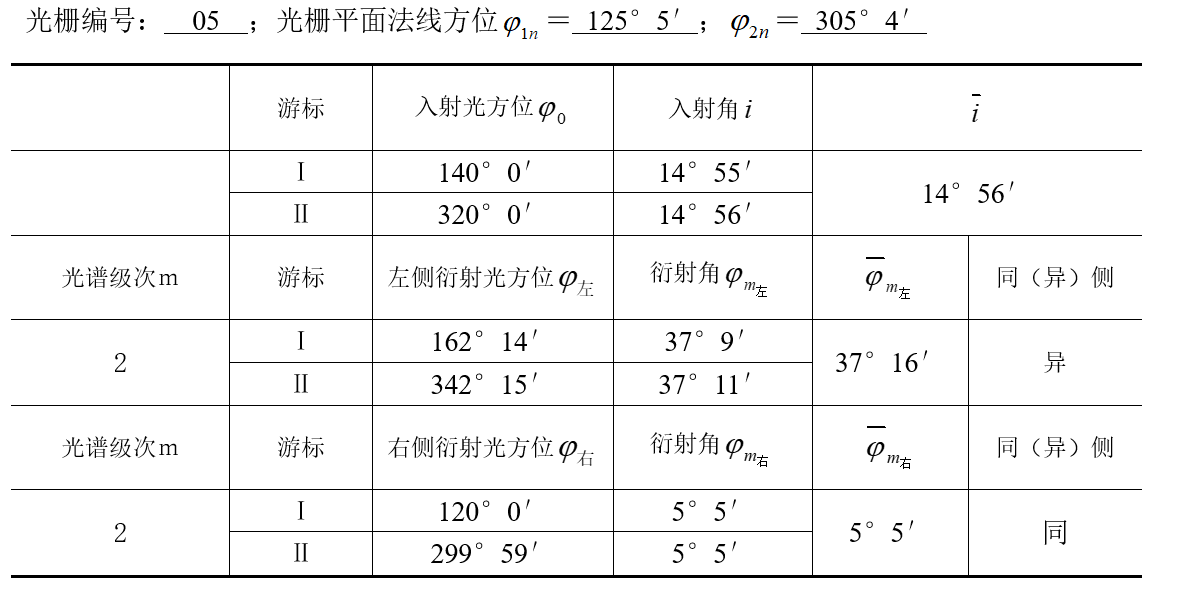
\includegraphics[scale=0.7]{表格2.png}
\end{figure}

由于$\varphi_{m \text{右}}=37^{\circ} 08^{\prime}$  与入射光线位于法线同侧,故:

$$
d\cdot \left(\sin \varphi_{m \text{右}}+\sin 15^{\circ}\right)=m \lambda
$$

故:
$$
\lambda=\frac{d (\sin \varphi_{m \text{右}}+\sin 15^{\circ})}{m}=578.4 \mathrm{~nm}
$$

偏差为:
$$
\delta = \frac{\lambda_{\mbox{黄2}}-\lambda}{\lambda_{\mbox{黄2}}}=0.23\%
$$

\subsection{用最小偏向角法测量波长较长的黄光波长}

\begin{figure}[H]
  \centering
  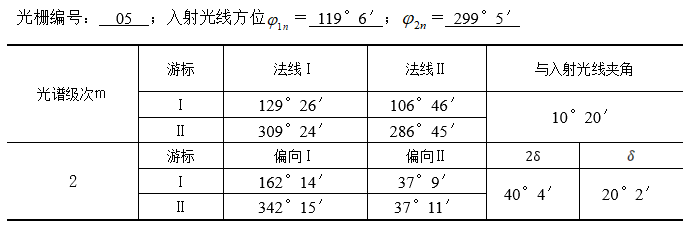
\includegraphics[scale=1.2]{表格3.png}
\end{figure}

由于:
$$
2d\sin \frac{\delta}{2} = m\lambda
$$

故:
$$
 \lambda=\frac{2d\sin \frac{\delta}{2}}{m}=579.1 nm
$$

偏差为:
$$
\delta = \frac{\lambda_{\mbox{黄1}}-\lambda}{\lambda_{\mbox{黄1}}}=0.0003\%
$$

可以看到此处与标准值相当接近。


\section{实验总结}

由于上个学期有过使用分光计的经历,再加上本次实验前有认真复习,故在本次实验中对于分光计的调节部分比较熟悉。由于分光计属于精密光学仪器,所以要在实验前对其进行望远镜调节、平行光管调节等操作。否则会给实验带来比较大的误差。

光栅实验中由于不能保证光栅底面和光学面垂直,故不需要对平台进行调水平,只需要在放上光栅后调节螺钉,使得光栅刻线垂直于分光计主轴。光栅的垂直入射则是利用了自准法,旋转小平台使得十字反射像和入射光线共线。

在实验中多次利用到了测量两倍物理量避免测量量相减求出单倍测量量的方法来减小误差,这点值得我注意,在今后的学习中可以加以实验和应用。

最后,感谢老师的悉心指导!

\section{原始数据及预习思考题}

\begin{figure}[H]
  \centering
  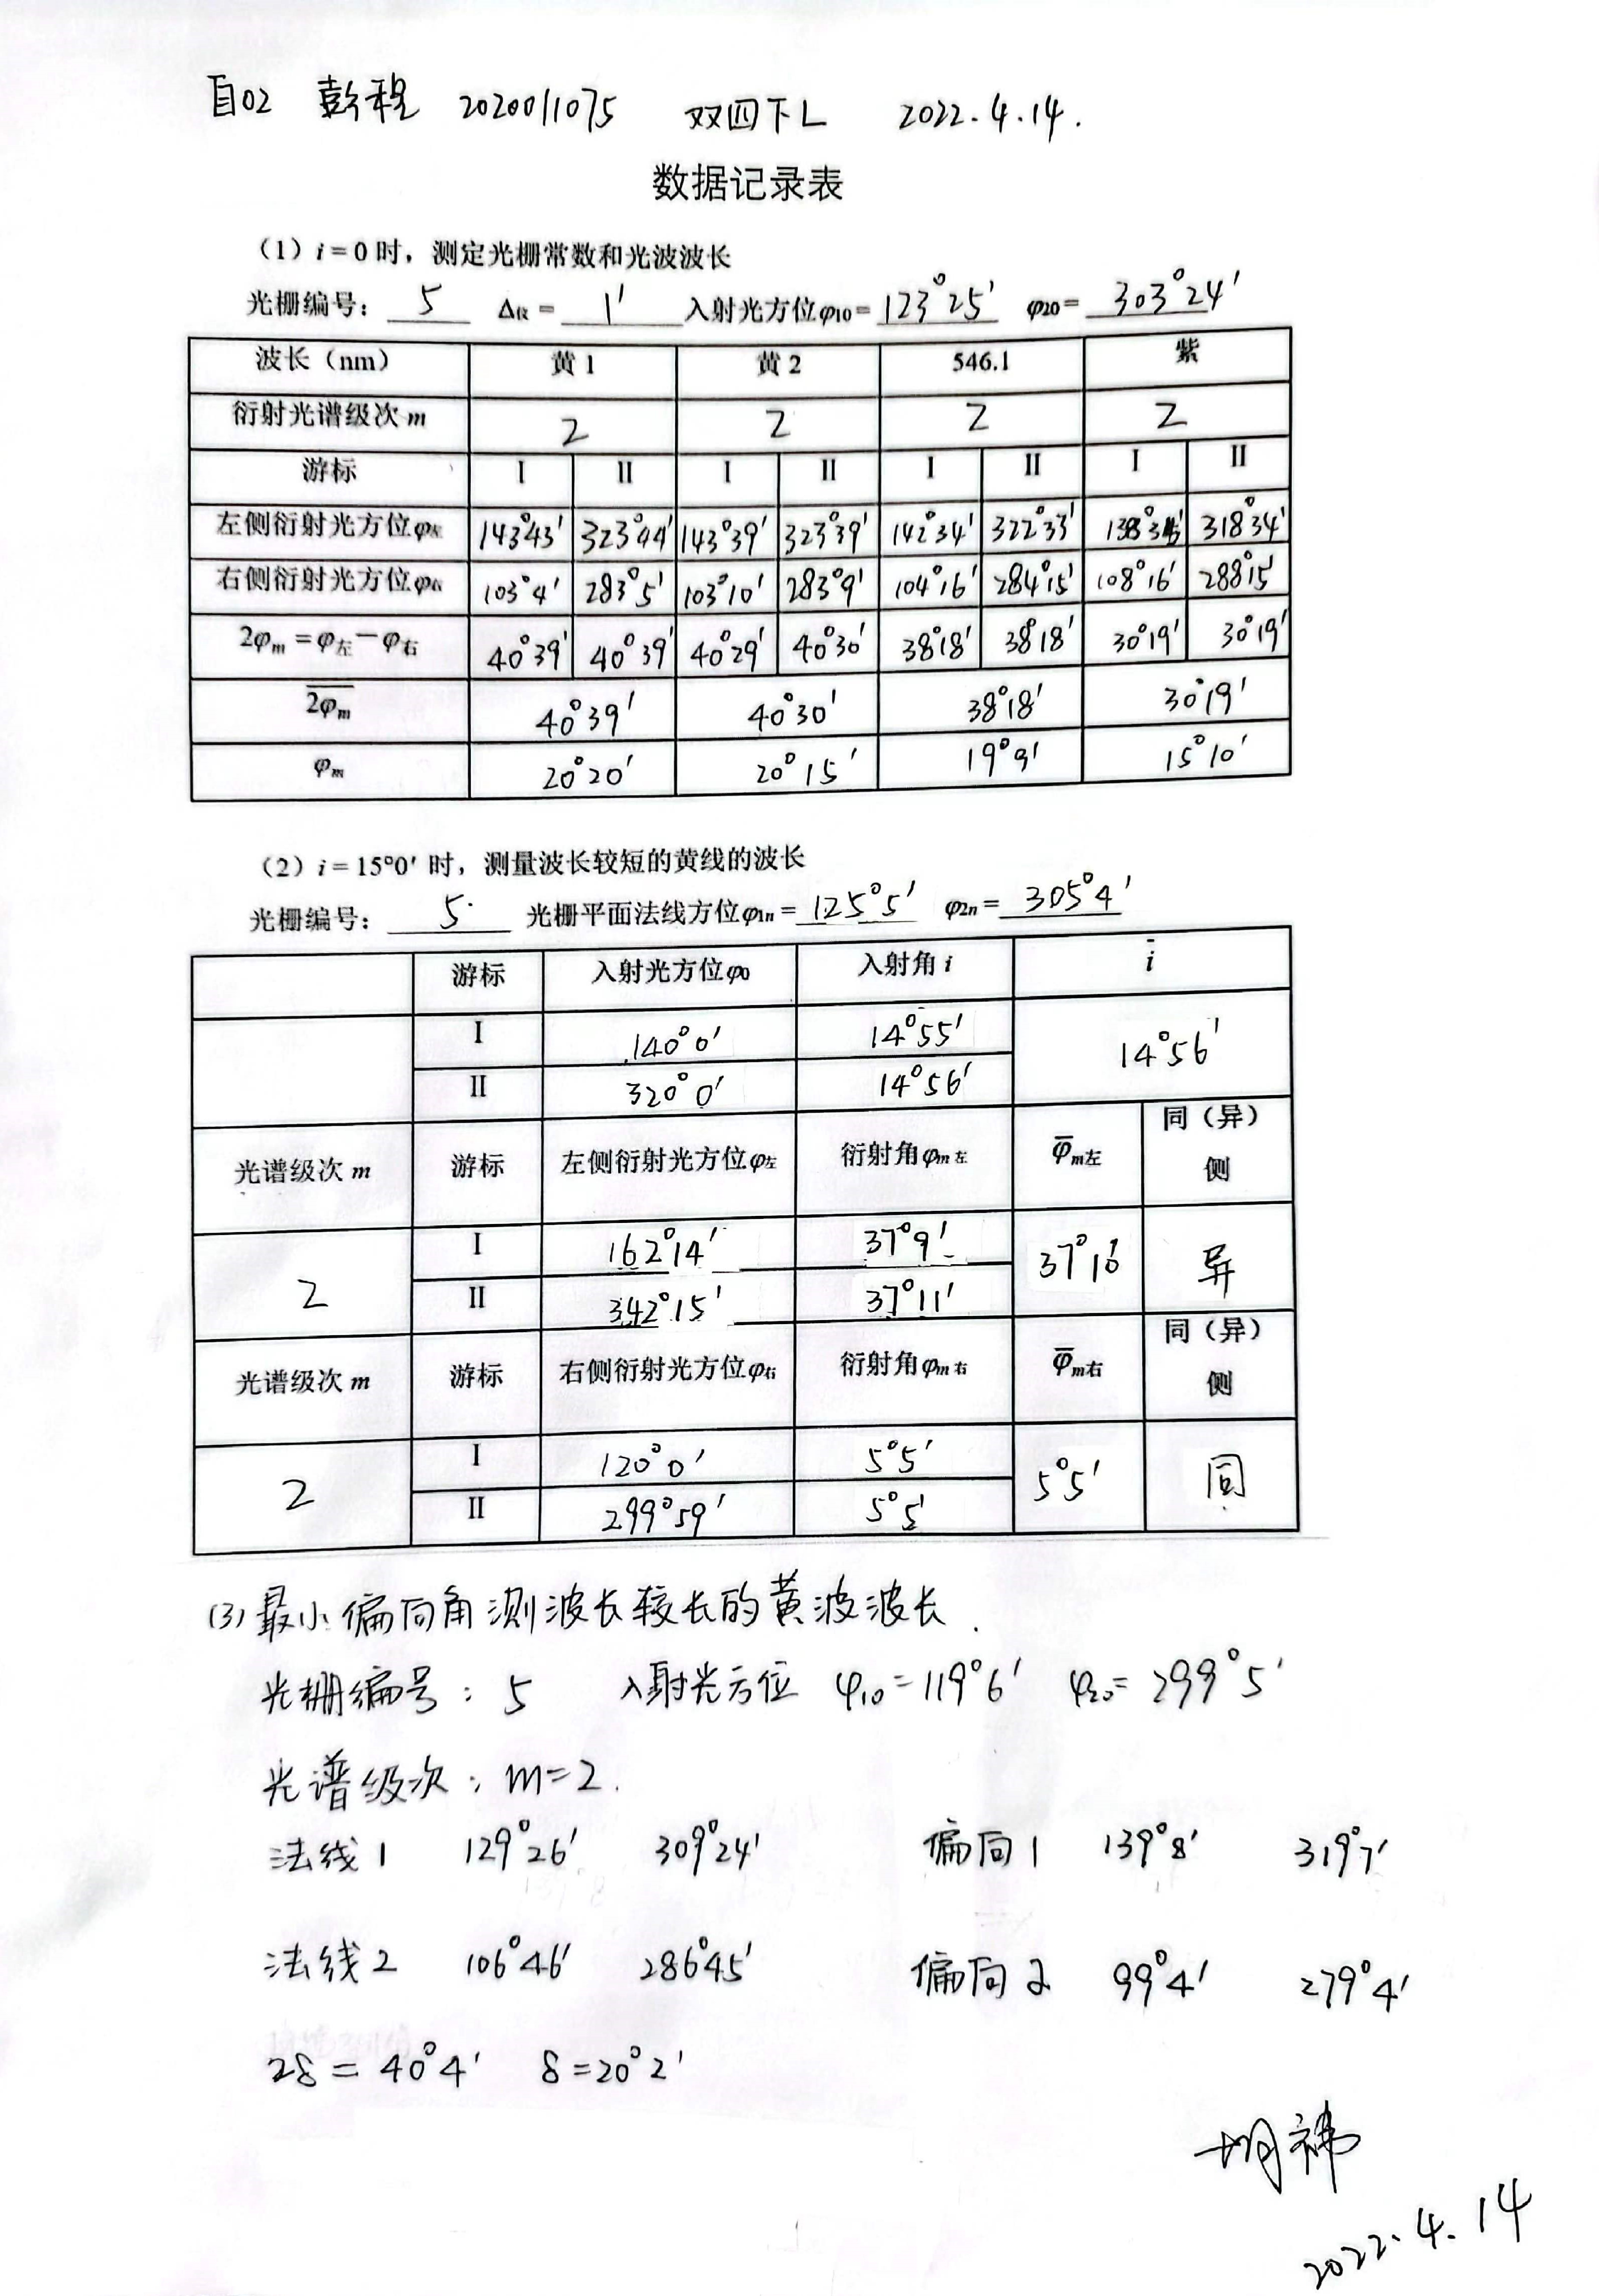
\includegraphics[scale=0.18]{数据.jpg}
\end{figure}

\begin{figure}[H]
  \centering
  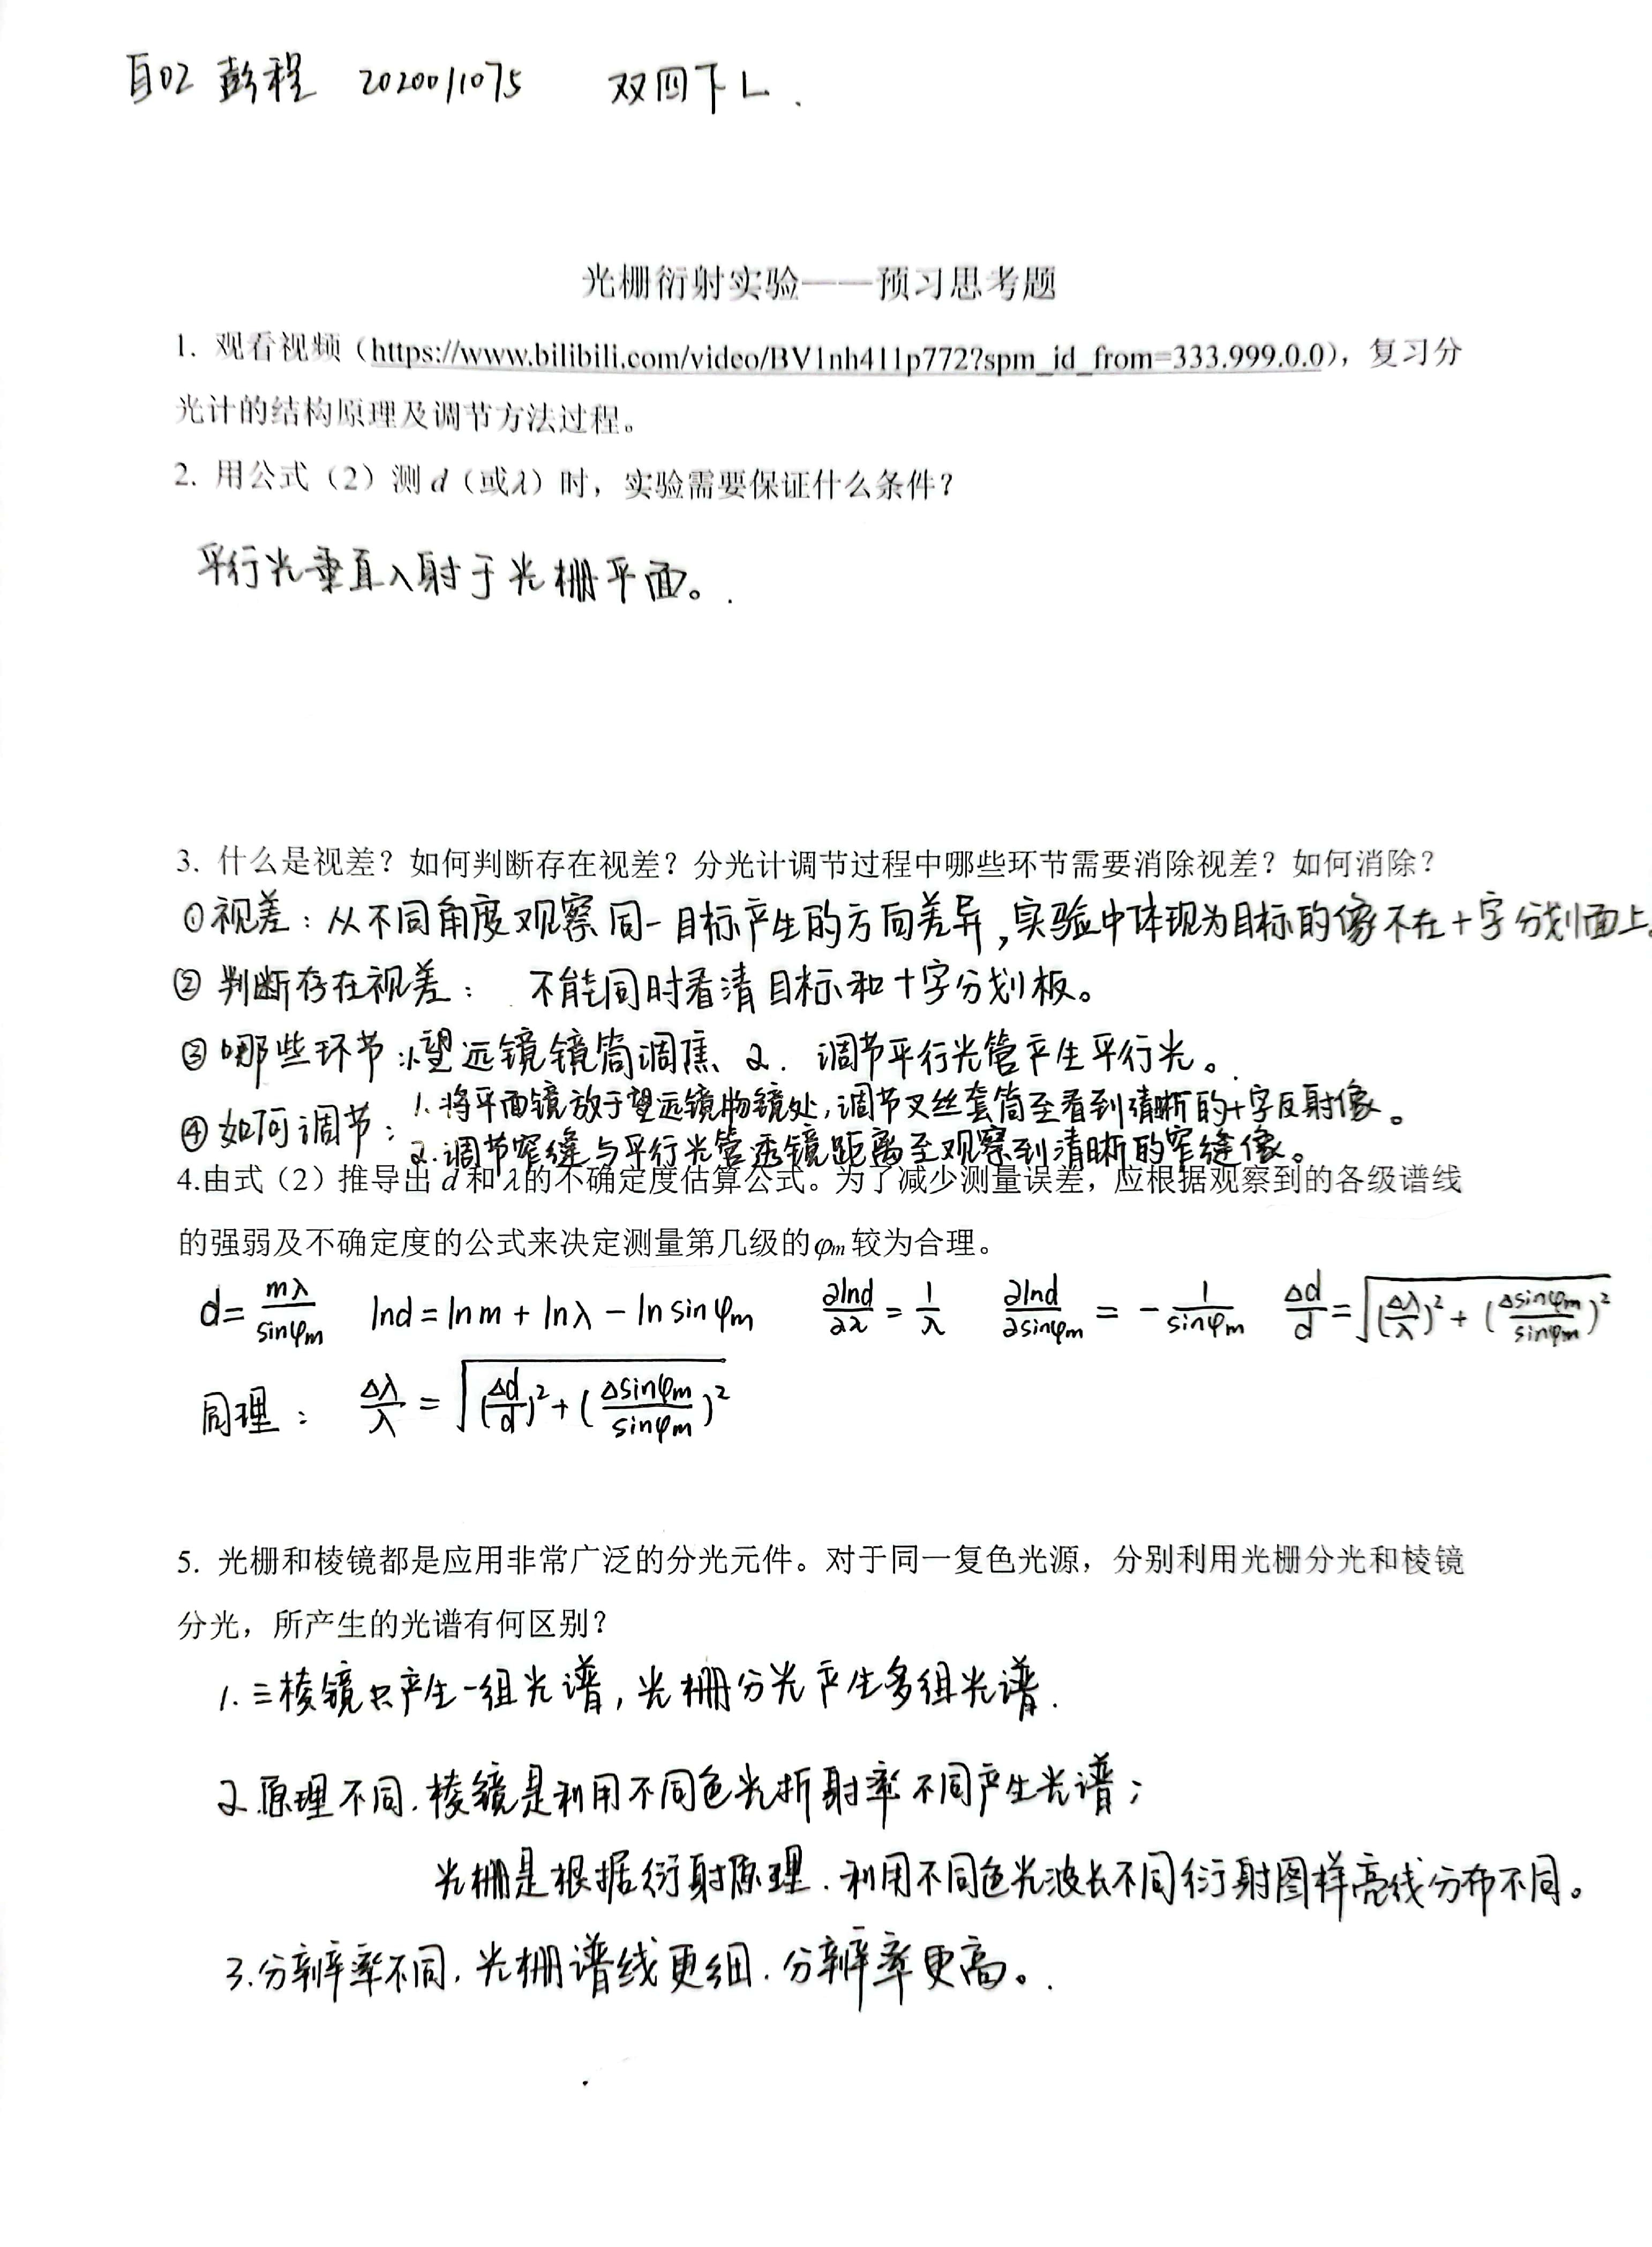
\includegraphics[scale=0.14]{预习.jpg}
\end{figure}

\end{document}